\chapter{Workshop and user testing}

\epigraph{Yeah you wanted a hit \\ but tell me \\ where's the point in it?}{You Wanted a Hit \\ LCD Soundsystem, 2010}

In the past I have taught several classes and crash courses of software of arts, and this experience informed my creation of the Tiny Trainable Instruments workshop. Teaching them was a way of user testing and releasing this thesis. In this chapter I explain the workshop design, feedback from the students, and what challenges we faced.

\section{Workshop design}

The Tiny Trainable Instruments workshop primary audience is artists and educators with no previous technical knowledge of programming, \acrshort{ML}, or microcontrollers. It is conceived as a hands-on experience, for people to build their own instruments, collect their own data, and train their own models.

The workshop consists of two sessions of two hours each, taught in two consecutive days for a total of four hours. The first session is focused on installation of the software, connecting the hardware components, and instruments using the color input. The second session is about capturing data and training models, for gesture detection.

This workshop was taught three times, the first two in English for people based in the U.S.A., and one last time in Spanish for people based in Chile. Each workshop had between six and seven students, for a total of twenty people participating.

The workshop was designed to be taught virtually or presentially. The participants require a laptop computer, internet connection, and a bill of materials for building the Tiny Trainable Instruments. To eliminate cost barriers, I applied and obtained a generous grant of 2,000.00 USD from the \acrlong{CAMIT}. This funding covered all the materials and shipping for the 20 participants, so that they could participate for free.

The workshop passed the required approval by the \acrshort{MIT} \acrfull{COUHES}. The workshop didn't ask students to identify themselves, or share any data, and they were always in control of their databases, so this activity complied with the required standards for testing on humans. Additionally, it was taught over videoconferencing software, so all health protocols were respected.

\section{Workshop promotion}


\begin{figure}[ht]
  \centering
  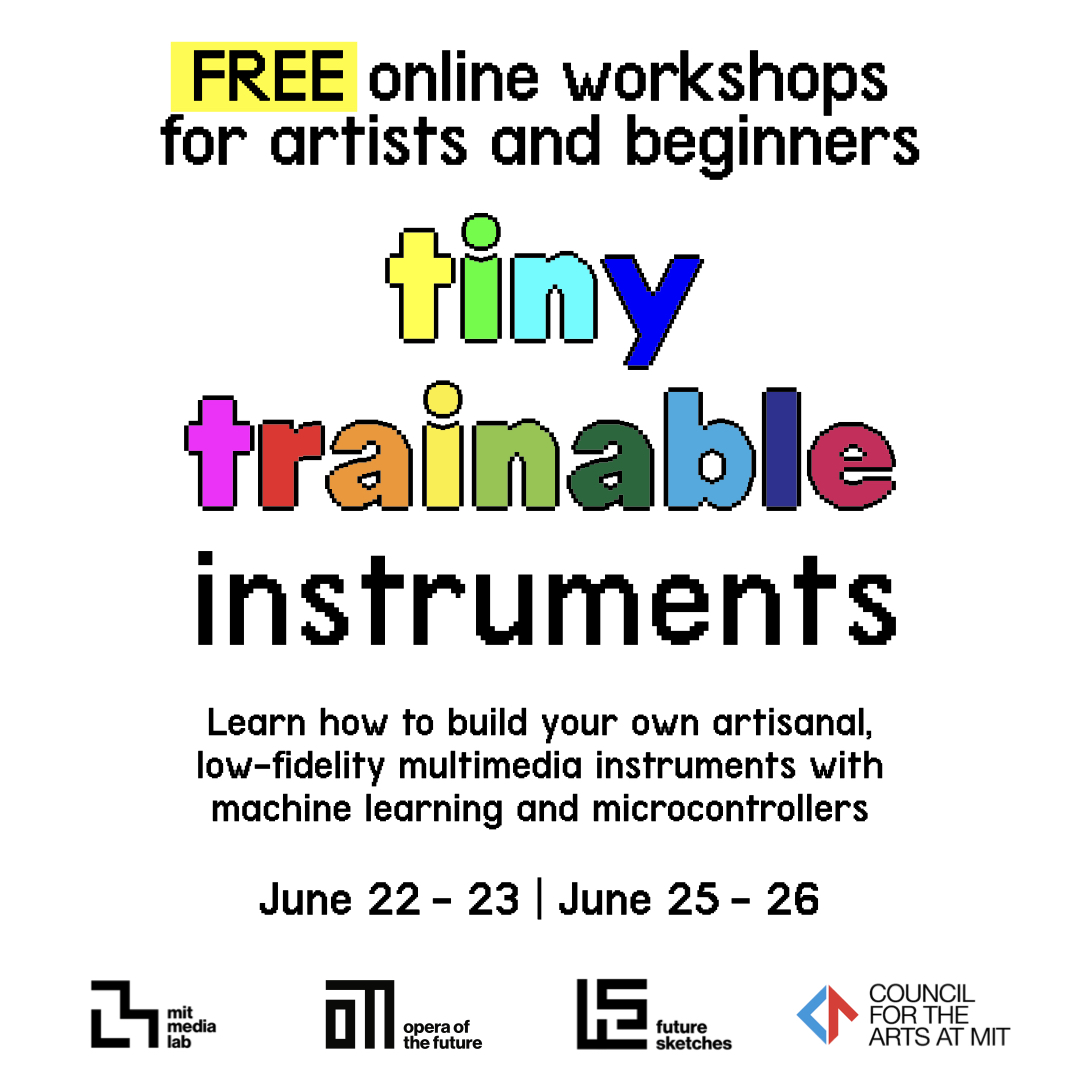
\includegraphics[width=0.75\linewidth,height=0.35\textheight,keepaspectratio]{images/workshop-en-1.jpg}
  \caption{Workshop flyer cover in English}
  \caption*{Graphics by Renata Gaui}
  \label{fig:workshop-english-flyer-page-1}
\end{figure}

\begin{figure}[ht]
  \centering
  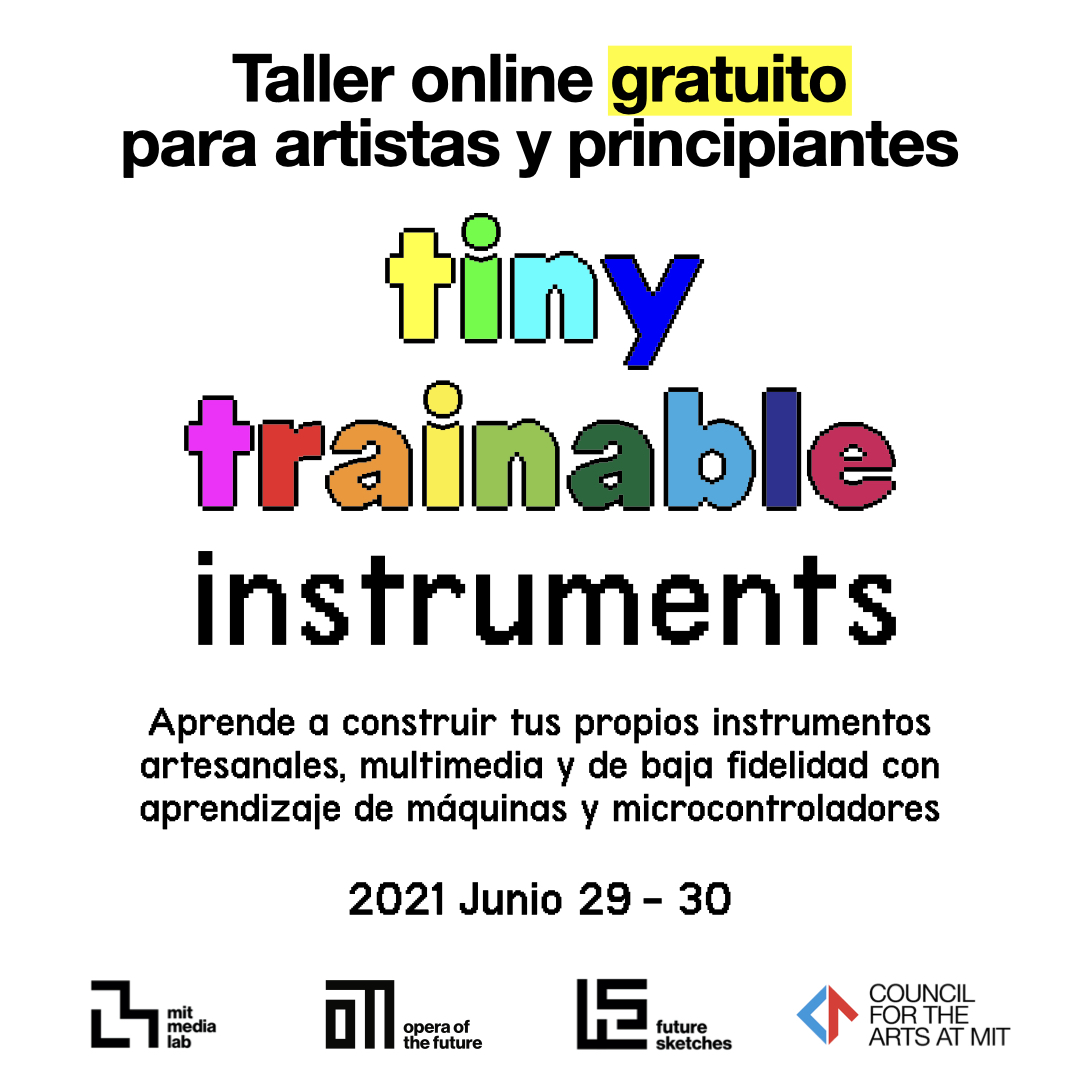
\includegraphics[width=0.75\linewidth,height=0.35\textheight,keepaspectratio]{images/workshop-es-1.jpg}
  \caption{Workshop flyer cover in Spanish}
  \caption*{Graphics by Renata Gaui}
  \label{fig:workshop-spanish-flyer-page-1}
\end{figure}



The multimedia aspect of this project was featured, in particular the ability to use different inputs, including color, gesture and speech, to control different outputs, including serial messages, sound, and motor movement.

\begin{figure}[ht]
  \centering
  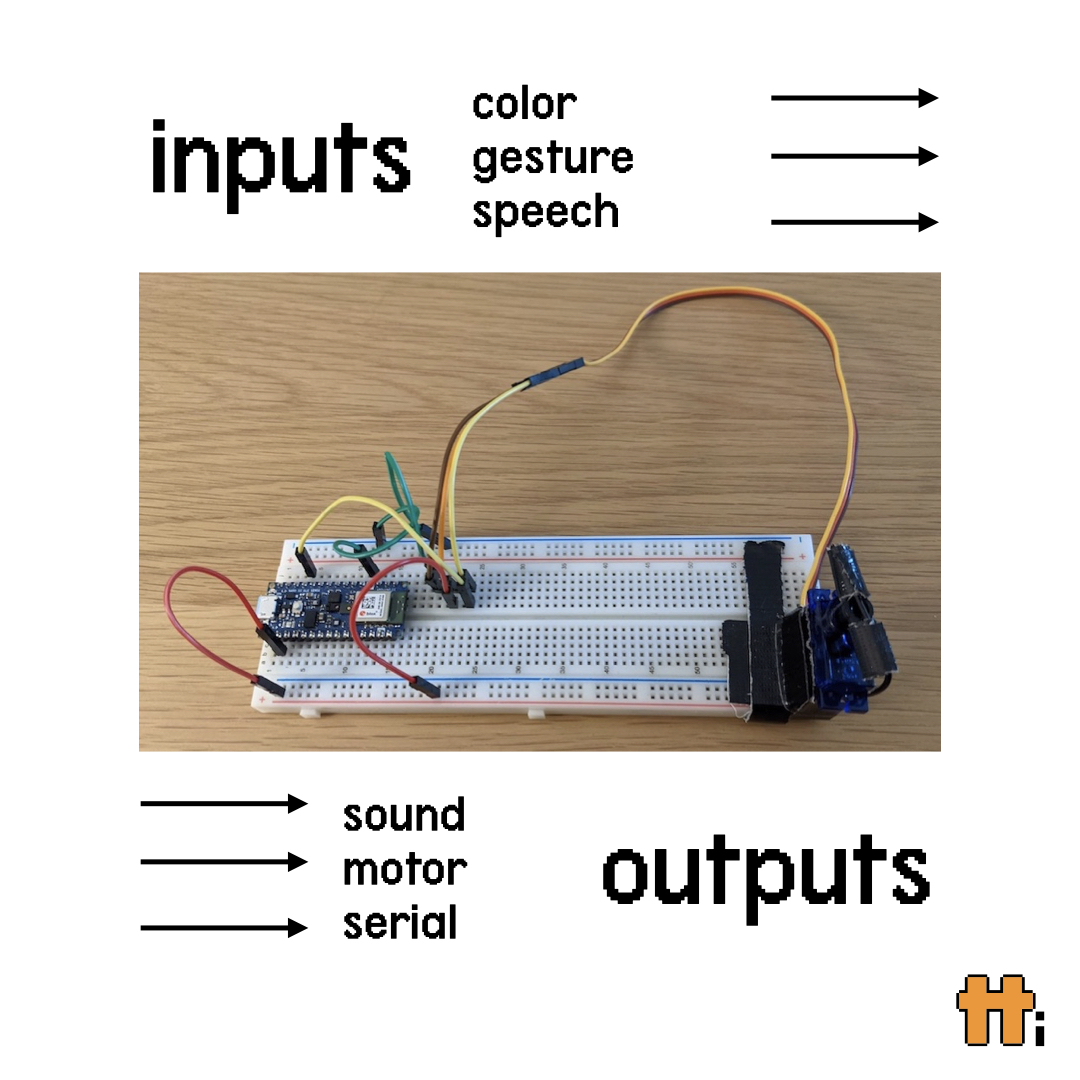
\includegraphics[width=0.75\linewidth,height=0.35\textheight,keepaspectratio]{images/workshop-en-2.jpg}
  \caption{Workshop multimedia output in English}
  \caption*{By Renata Gaui}
  \label{fig:workshop-english-flyer-page-2}
\end{figure}

\begin{figure}[ht]
  \centering
  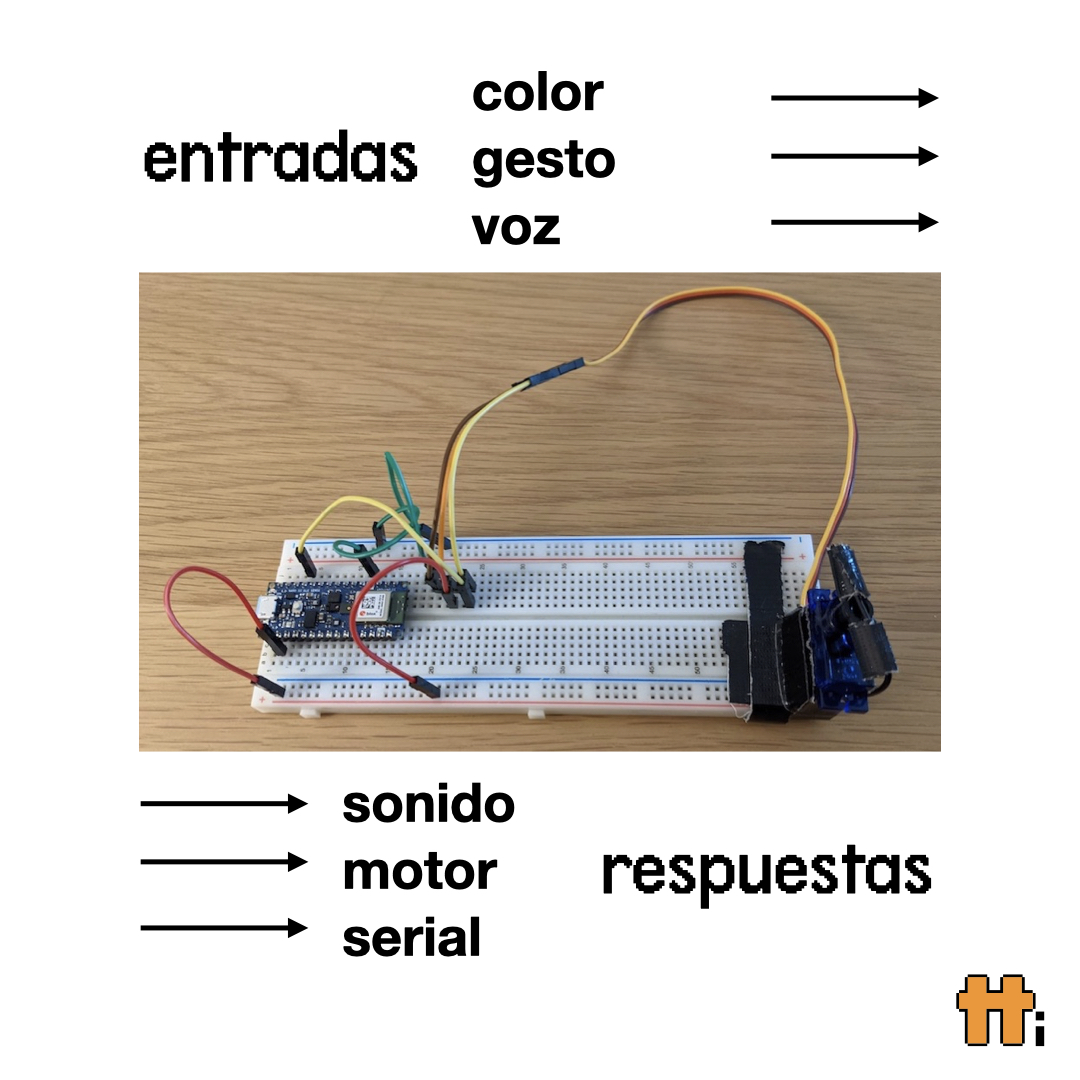
\includegraphics[width=0.75\linewidth,height=0.35\textheight,keepaspectratio]{images/workshop-es-2.jpg}
  \caption{Workshop multimedia output in Spanish}
  \caption*{By Renata Gaui}
  \label{fig:workshop-spanish-flyer-page-2}
\end{figure}

\section{Workshop structure}

In the first session we will first help people with installation of the software, and then move on to start wiring the materials on the electronic breadboard material. We will concentrate on the simpler examples with color input. We will also collect data of gesture and speech to create custom databases and use them to train other slow machine learning models that will keep on running on the student's workshops after the workshop is over.

In the second session we will use the result of the trained models to create more advanced instruments that react to gesture and speech. We will also show the participants the other 

I applied to and was awarded a grant by the Council for the arts at MIT (CAMIT), which consisted of 2,000.00 USD to buy materials to teach the Tiny Trainable Instruments workshop to 20 people, during June 2021.


what did participants create

what challenges did they face

what did they find most interesting

\section{Workshop feedback}

After the completion of the workshops I sent the students a Google form to ask for anonymous feedback. Here are some of the results.

Students called the workshop interesting, challenging, fun, innovative, inspiring, didactical, exciting, fun, new, fast-paced, and experimental.


what changes did they suggest, etc.

Did the workshops provide you with new ideas on how to modify the TinyTrainable library in the future? Or new ideas on how to introduce the library to beginners?

\begin{figure}[ht]
  \centering
  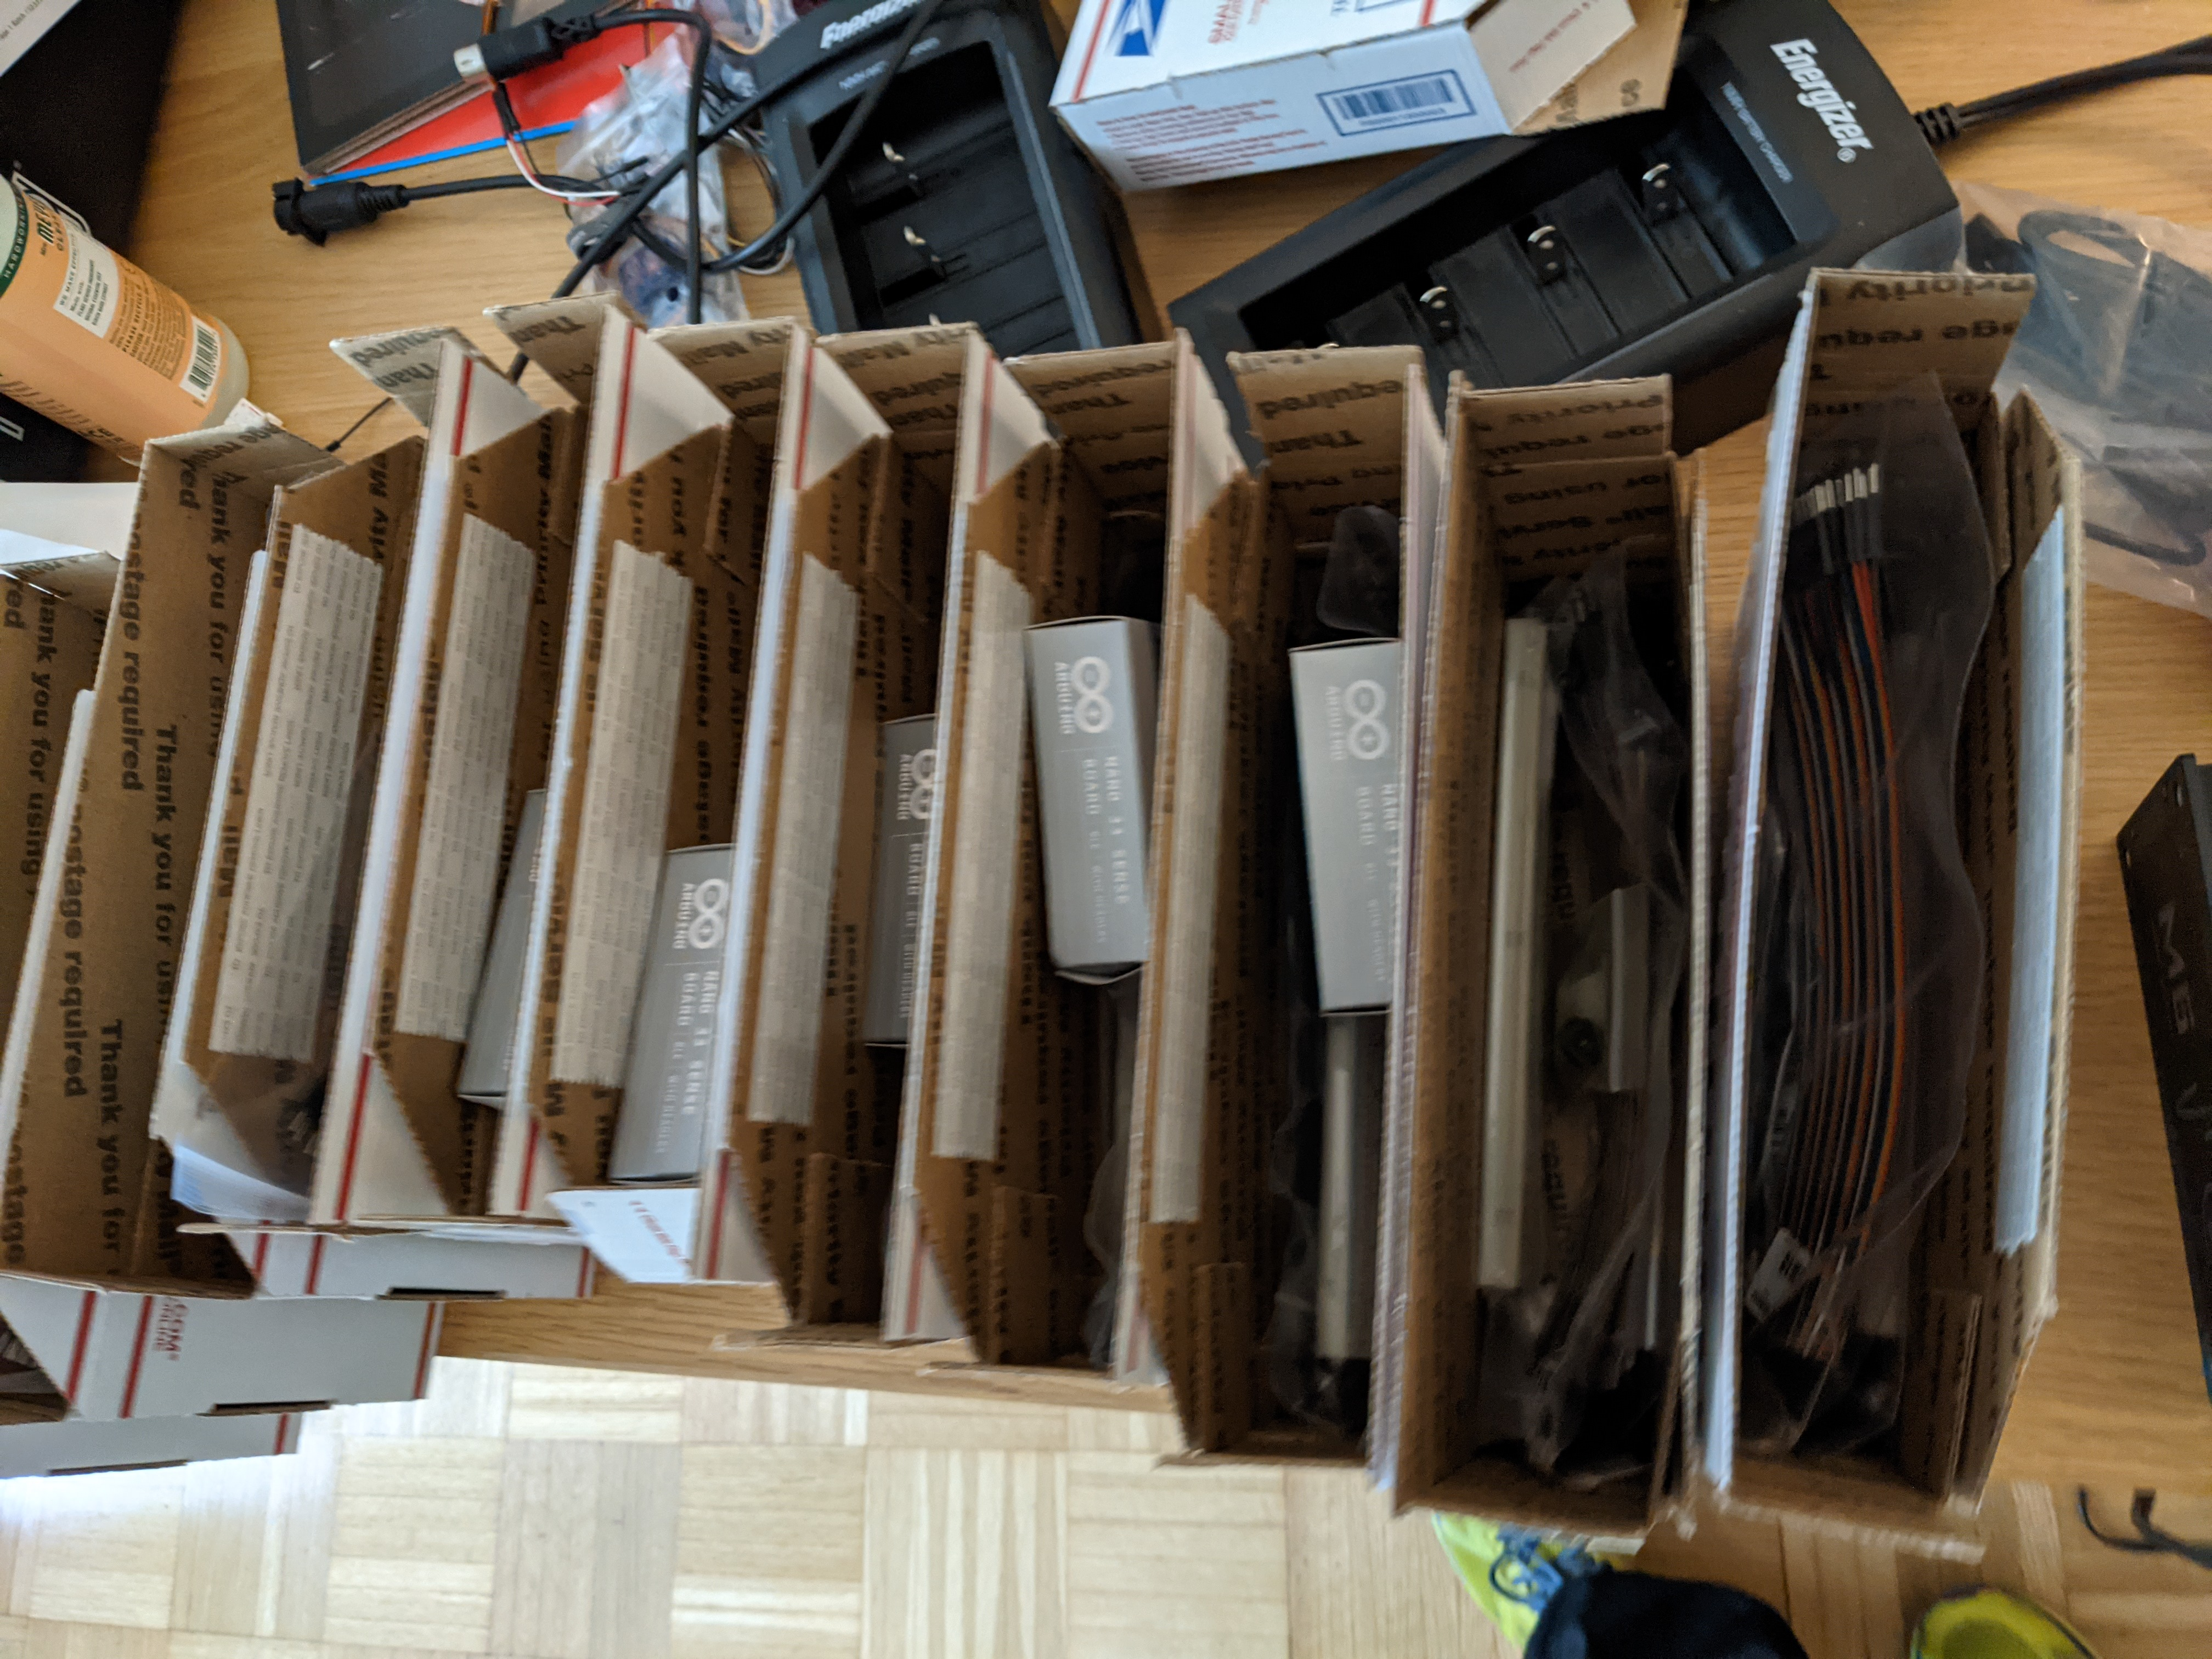
\includegraphics[width=0.75\linewidth,height=0.25\textheight,keepaspectratio]{images/workshop-packages.jpg}
  \caption{Workshop packages}
  \caption*{Picture by myself}
  \label{fig:workshop-packages}
\end{figure}

The workshop instructions are documented on the docs/ folder of the repository available at \url{https://github.com/montoyamoraga/tiny-trainable-instruments}

Each workshop consists of 2 sessions of 2 hours each, spread over 2 consecutive days.


\section{Multimedia documentation}

TODO: upload a collection of examples made by people who came to the workshops, featuring the software library and what they learned.
